\chapter{Contexte métier : le groupe, information produit et généralités sur les données}
    \label{business_chap}
    \large
    L'objet de l'ensemble de cette annexe est de donner sur le Groupe Pomona et la gestion de l'information produit. des éclairages nécessaires à la compréhension du cas d'usage développé.
    Bien d'autres aspects sur la société, pourraient être mentionnés (ex : des indicateurs sur l'activité, l'histoire du groupe\dots) mais ils seront omis car non indispensables à la compréhension du sujet.
    Plus de détails sur le groupe sont accessibles sur le site web de la société\cite{site_pomona}.
    \normalsize   

    \section{Description du groupe}

 

        \subsection{Le métier du Groupe Pomona}
        \label{business}

        Le Groupe Pomona est une société de distribution livrée de produits alimentaires à destination des professionnels des métiers de bouche.
        L'activité du groupe consiste uniquement à acheter et revendre de la marchandise, à l'exclusion de toute activité de fabrication ou de transformation\footnote{de très rares cas de transformation existent (ex : mûrissage de fruits, filetage de poisson) mais sont extrêmement exceptionnels}. Le groupe Pomona est une société de \emph{distribution}. Elle ne possède d'ailleurs pas d'actif industriel (autre que des entrepôts logistiques) ni d'agréement pour transformer les marchandises.        
        
        Cette activité d'achat/vente se fait dans la majorité des cas sous le régime du \emph{négoce}, à savoir que le groupe acquiert la propriété des marchandises qu'il commercialise avant de la céder à ses clients.
        L'autre régime est celui dit de la \emph{prestation (logistique)}.
        Dans ce cas, par le jeux d'écritures comptables, la valorisation du stock disparaît des comptes du groupe.
        Néanmoins, indépendamment de cet aspect purement comptable, l'ensemble :
        \begin{description}
            \item[des flux de documents :] commandes d'achat, factures fournisseur, commandes de vente, factures clients
            \item[des flux financiers :] paiements fournisseur, paiements client
            \item[des flux physiques :] réception et stockage, préparation et expédition
        \end{description}
        restent largement inchangés.
        
        Pour résumer, l'activité de l'ensemble des entités du groupe pourraient se résumer via le schéma présenté à la \reffig{fig:flux metier}

        \begin{figure}[htbp]
            \begin{center}
            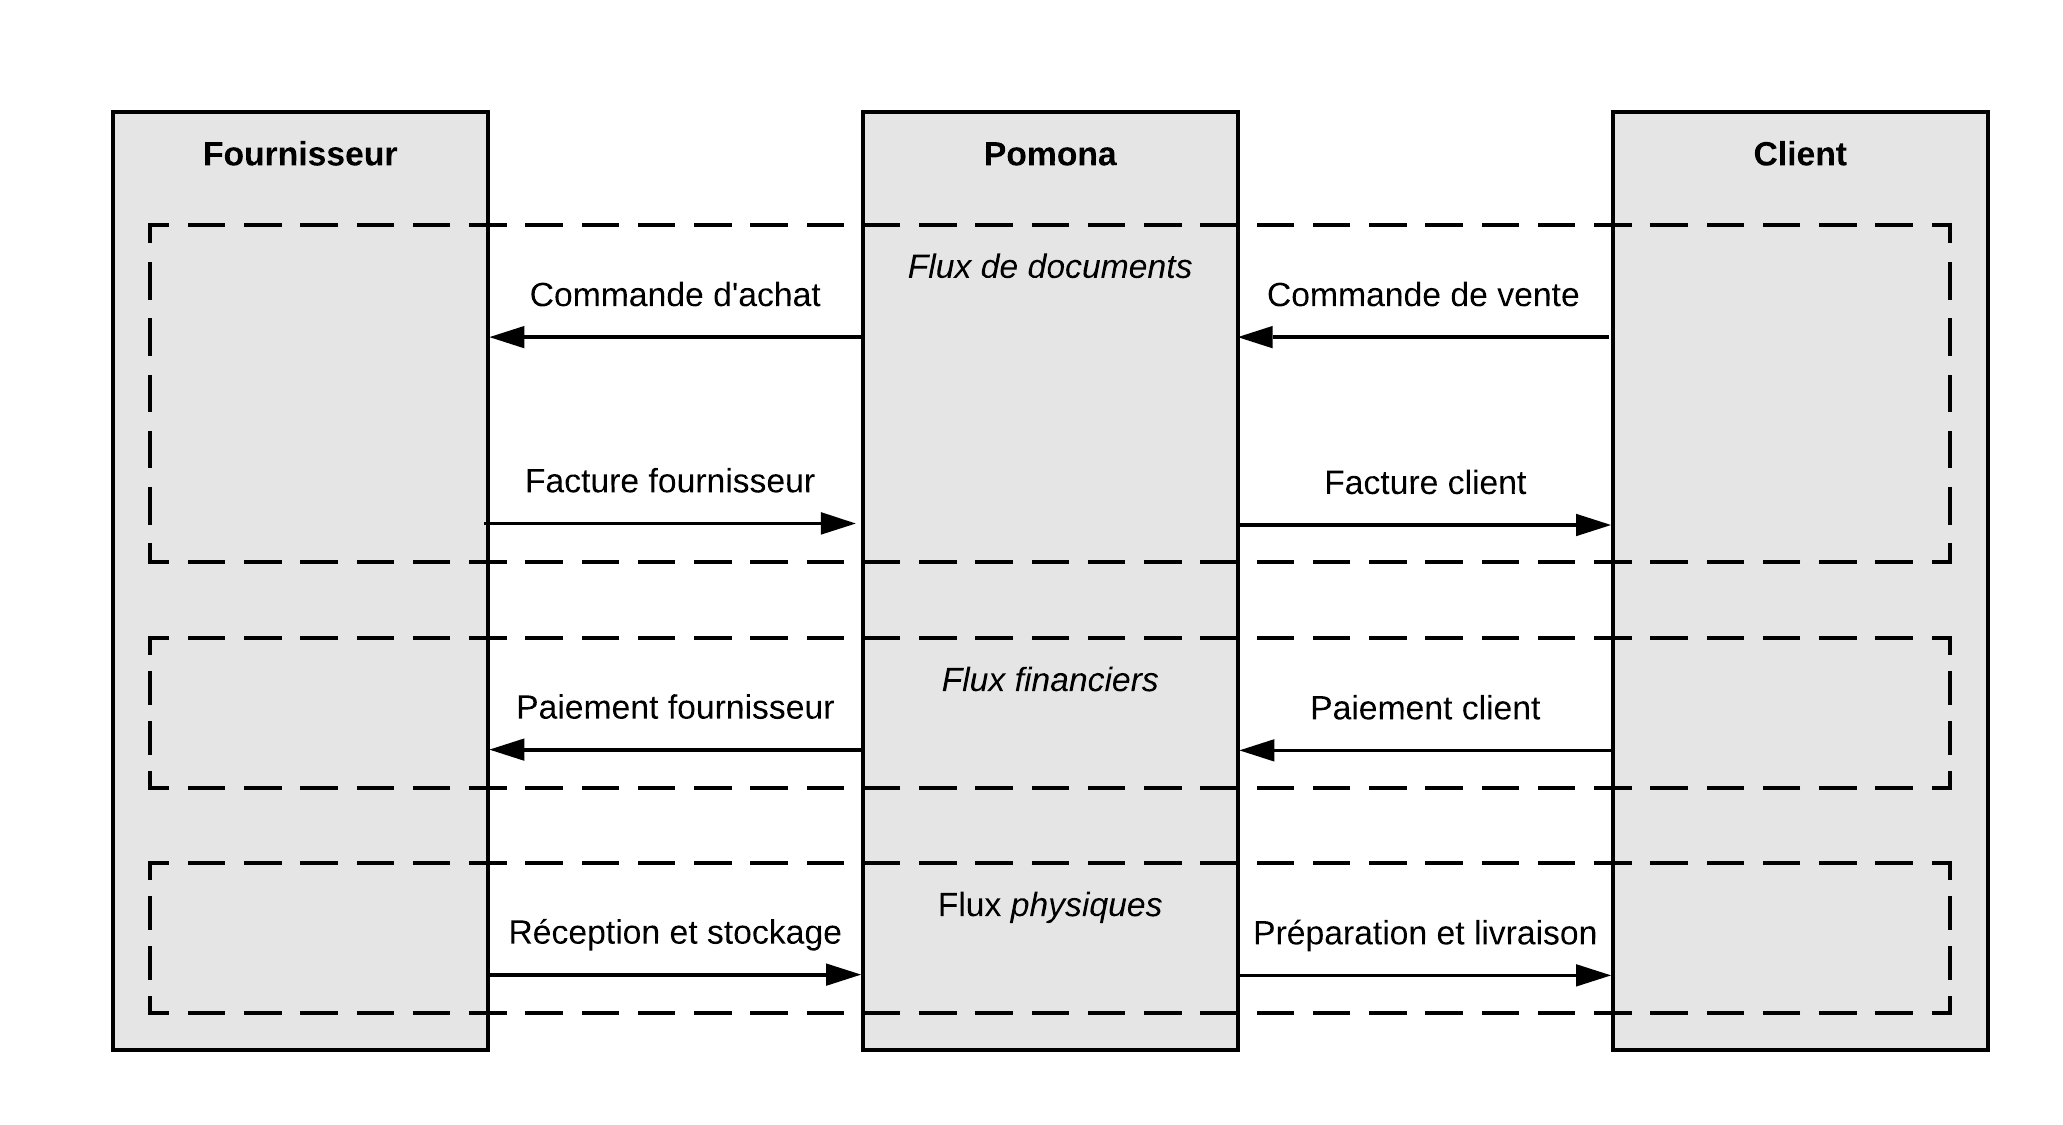
\includegraphics[width=\linewidth]{img/Les flux metier de Pomona.png}
            \end{center}
            \caption{Les flux métier avec les partenaires commerciaux}
            \label{fig:flux metier}
        \end{figure}

        \emphbox{Le métier du groupe est d'être un \emph{grossiste}, qui achète et revend des produits alimentaires\footnotemark \ \emph{sans produire ou transformer quoi que ce soit}.}
        \footnotetext{dans la grande majorité des cas, cf. \emph{Les produits non-alimentaires} \mref{produits_nonal}}

        \subsection{La décentralisation}
        
        Le Groupe Pomona est un groupe fortement décentralisé, avec des organisations largement indépendantes les unes des autres. 

            \subsubsection{Les Directions fonctionnelles}
            \label{les_directions_fonctionnelles}

            Pour des raisons évidentes de recherche de synergies ou de conformité réglementaires, certaines activités restent toutefois mutualisées à la maille du groupe.
            Il s'agit des organisations suivantes :
            \begin{description}
                \item[La Direction Administrative et Financière (DAF) :] regroupe les équipes comptables groupe, l'audit interne et la consolidation financière
                \item[La Direction Qualité Sécurité et Environnement (DQSE) :] est en charge de définir et contrôler l'application des standard de qualité
                \item[La Direction des Systèmes d'Information (DSI) :] développe et maintient en condition opérationnelles les systèmes d'information du groupe
                \item[La Direction Technique et Logistique (DTL) :] est en charge des projets immobiliers (entrepôts), des négociations avec les transporteurs et joue un rôle de conseil interne sur les sujets logistiques
                \item[La Direction des Ressources Humaines :] se charge de l'ensemble des aspects en lien avec le recrutement, la paye et les sujets sociaux
                \item[La Direction Commerciale groupe (DCG) :] définit une stratégie et des bonnes pratiques commerciales et marketing
            \end{description}

            \subsubsection{Les clients du groupe}
            \label{clients}

            Afin de comprendre l'organisation du groupe, il est nécessaire de connaître la typologie de ses clients.
            Comme mentionné précédemment, le groupe s'adresse exclusivement aux professionnels des métiers de bouche.
            Aucune marchandise n'est vendue à des particuliers.
            Les principales typologies de clients sont les suivantes : 
            \begin{description}
                \item[Les Sociétés de Restauration :] elles exploitent les restaurants d'entreprise, certaines cantines d'établissements d'enseignement, les maisons de retraite, \dots
                \item[Les Marchés Publics :] regroupent les clients qui dépendent des collectivités (écoles, hôpitaux, prisons, \dots)
                \item[La restauration commerciale :] est l'ensemble des restaurants à vocation commerciale, qu'ils soient chaînés (hippopotamus, O'Tacos, \dots) ou indépendants (\og le restaurant du coin \fg)
                \item[Les spécialistes :] il s'agit des détaillants spécialisés qui s'adressent aux particuliers. Boulangers, pâtissiers, bouchers, traiteurs, vente à emporter, \dots
                \item[Les Grandes et Moyennes surfaces (la GMS) :] sont les enseignes de la grande distribution. En général, l'accès à ces clients est compliqué par les règles mises en place par leurs centrales d'achat. Il représentent en général qu'un canal de vente d'opportunité.
            \end{description}

            Les trois premières de ces catégories représentent ce que l'on appelle la \emph{Restauration Hors Domicile (RHD)} (ou parfois également la Restauration Hors Foyer, RHF).

            \subsubsection{Premier niveau de décentralisation : les branches}
            \label{les_branches}
            Le Groupe Pomona est divisé en branches, qui sont des unités opérationnelles indépendantes, et qui ont toute latitude pour gérer leurs stratégie et politique commerciales, la gestion de leurs achats, leur stratégie marketing, \dots
            En particulier, les systèmes d'information ne sont pas identiques entre les différentes branches.
            Afin d'éviter de se concurrencer entre elles, leurs domaines d'activité respectifs ont été partitionnés par familles de produit commercialisés, segments client cibles et géographie. 

                \paragraph{Les branches RHD}
                
                Les branches RHD s'adressent aux client de la Restauration Hors Domicile (cf. section \mref{clients}) en France.
                Elles se répartissent ce marché en travaillant des gammes de produits distinctes.
                Il s'agit des branches historiques du groupe, qui représentent l'essentiel de son chiffre d'affaire.
                La répartition par produit est la suivante :
                \begin{description}
                    \item[PassionFroid :] spécialiste des \emph{produits surgelés, de la viande fraîche et des produits laitiers}
                    \item[\'{E}piSaveurs :] spécialiste des produits qui se conservent à température ambiante : \emph{produits d'épicerie, conserves, boissons et consommables de cuisine non-alimentaires}
                    \item[TerreAzur :] spécialites des \emph{Fruits et Légumes frais, et Produits De la Mer frais} 
                \end{description}
                La non-concurrence entre les branches est assurée par le fait qu'elles ne commercialisent pas les mêmes produits.
                Bien que nommées RHD, elles peuvent également vendre leurs produits à la grande distribution (GMS : Grandes et Moyennes Surfaces), mais généralement ces marchés sont verrouillés par les centrales d'achat des grandes enseignes.
                La branche TerreAzur arrive toutefois à prendre des parts de marché significatives sur ce segment.
                Les branches RHD utilisent le progiciel SAP comme système de gestion.
                La branche TerreAzur est en cours de déploiement, en 2020 environ les 2 tiers des succursales travaillent avec ce progiciel.

                \paragraph{Les branches spécialistes}

                Les branches spécialistes s'adressent aux clients dits spécialistes (cf. section \mref{clients}) en France.
                Elles sont en mesure de commercialiser tout type de produit pour répondre aux besoins de leurs clients.
                En particulier, elles peuvent tout à fait commercialiser certains produits qui sont également vendus par les branches RHD.
                Elles se répartissent la clientèle spécialiste de la manière suivante :
                \begin{description}
                    \item[Délice et Création :] s'addresse aux \emph{Boulangers et Pâtissiers}
                    \item[Saveurs d'Antoine :] s'adresse aux \emph{Bouchers, Charcutiers et Traiteurs}
                    \item[Relais d'Or :] s'addresse à la \emph{restauration commerciale indépendante}
                \end{description}
                Comme pour les branches RHD, ces branches peuvent lorsqu'elles en ont l'opportunité vendre leurs produits à la GMS.

                \paragraph{L'étranger}

                Bien que le Groupe Pomona soit une société dont l'essentiel de l'activité est faite sur le marché français, deux réseaux sont en cours de constitution sur des pays limitrophe.
                Ces branches sont susceptibles de travailler tout type de produit, à destination de tout type de client.
                Elles sont positionnées sur les marchés suivants : 
                \begin{description}
                    \item[Pomona Suisse :] présente sur le marché Suisse
                    \item[Pomona Iberia :] présente sur le marché Espagnol 
                \end{description}

                On peut synthétiser la répartition de l'activité par branche de la manière présentée à la \reffig{fig:repartition_activite}.

                \begin{figure}[htpb]
                    \begin{center}
                    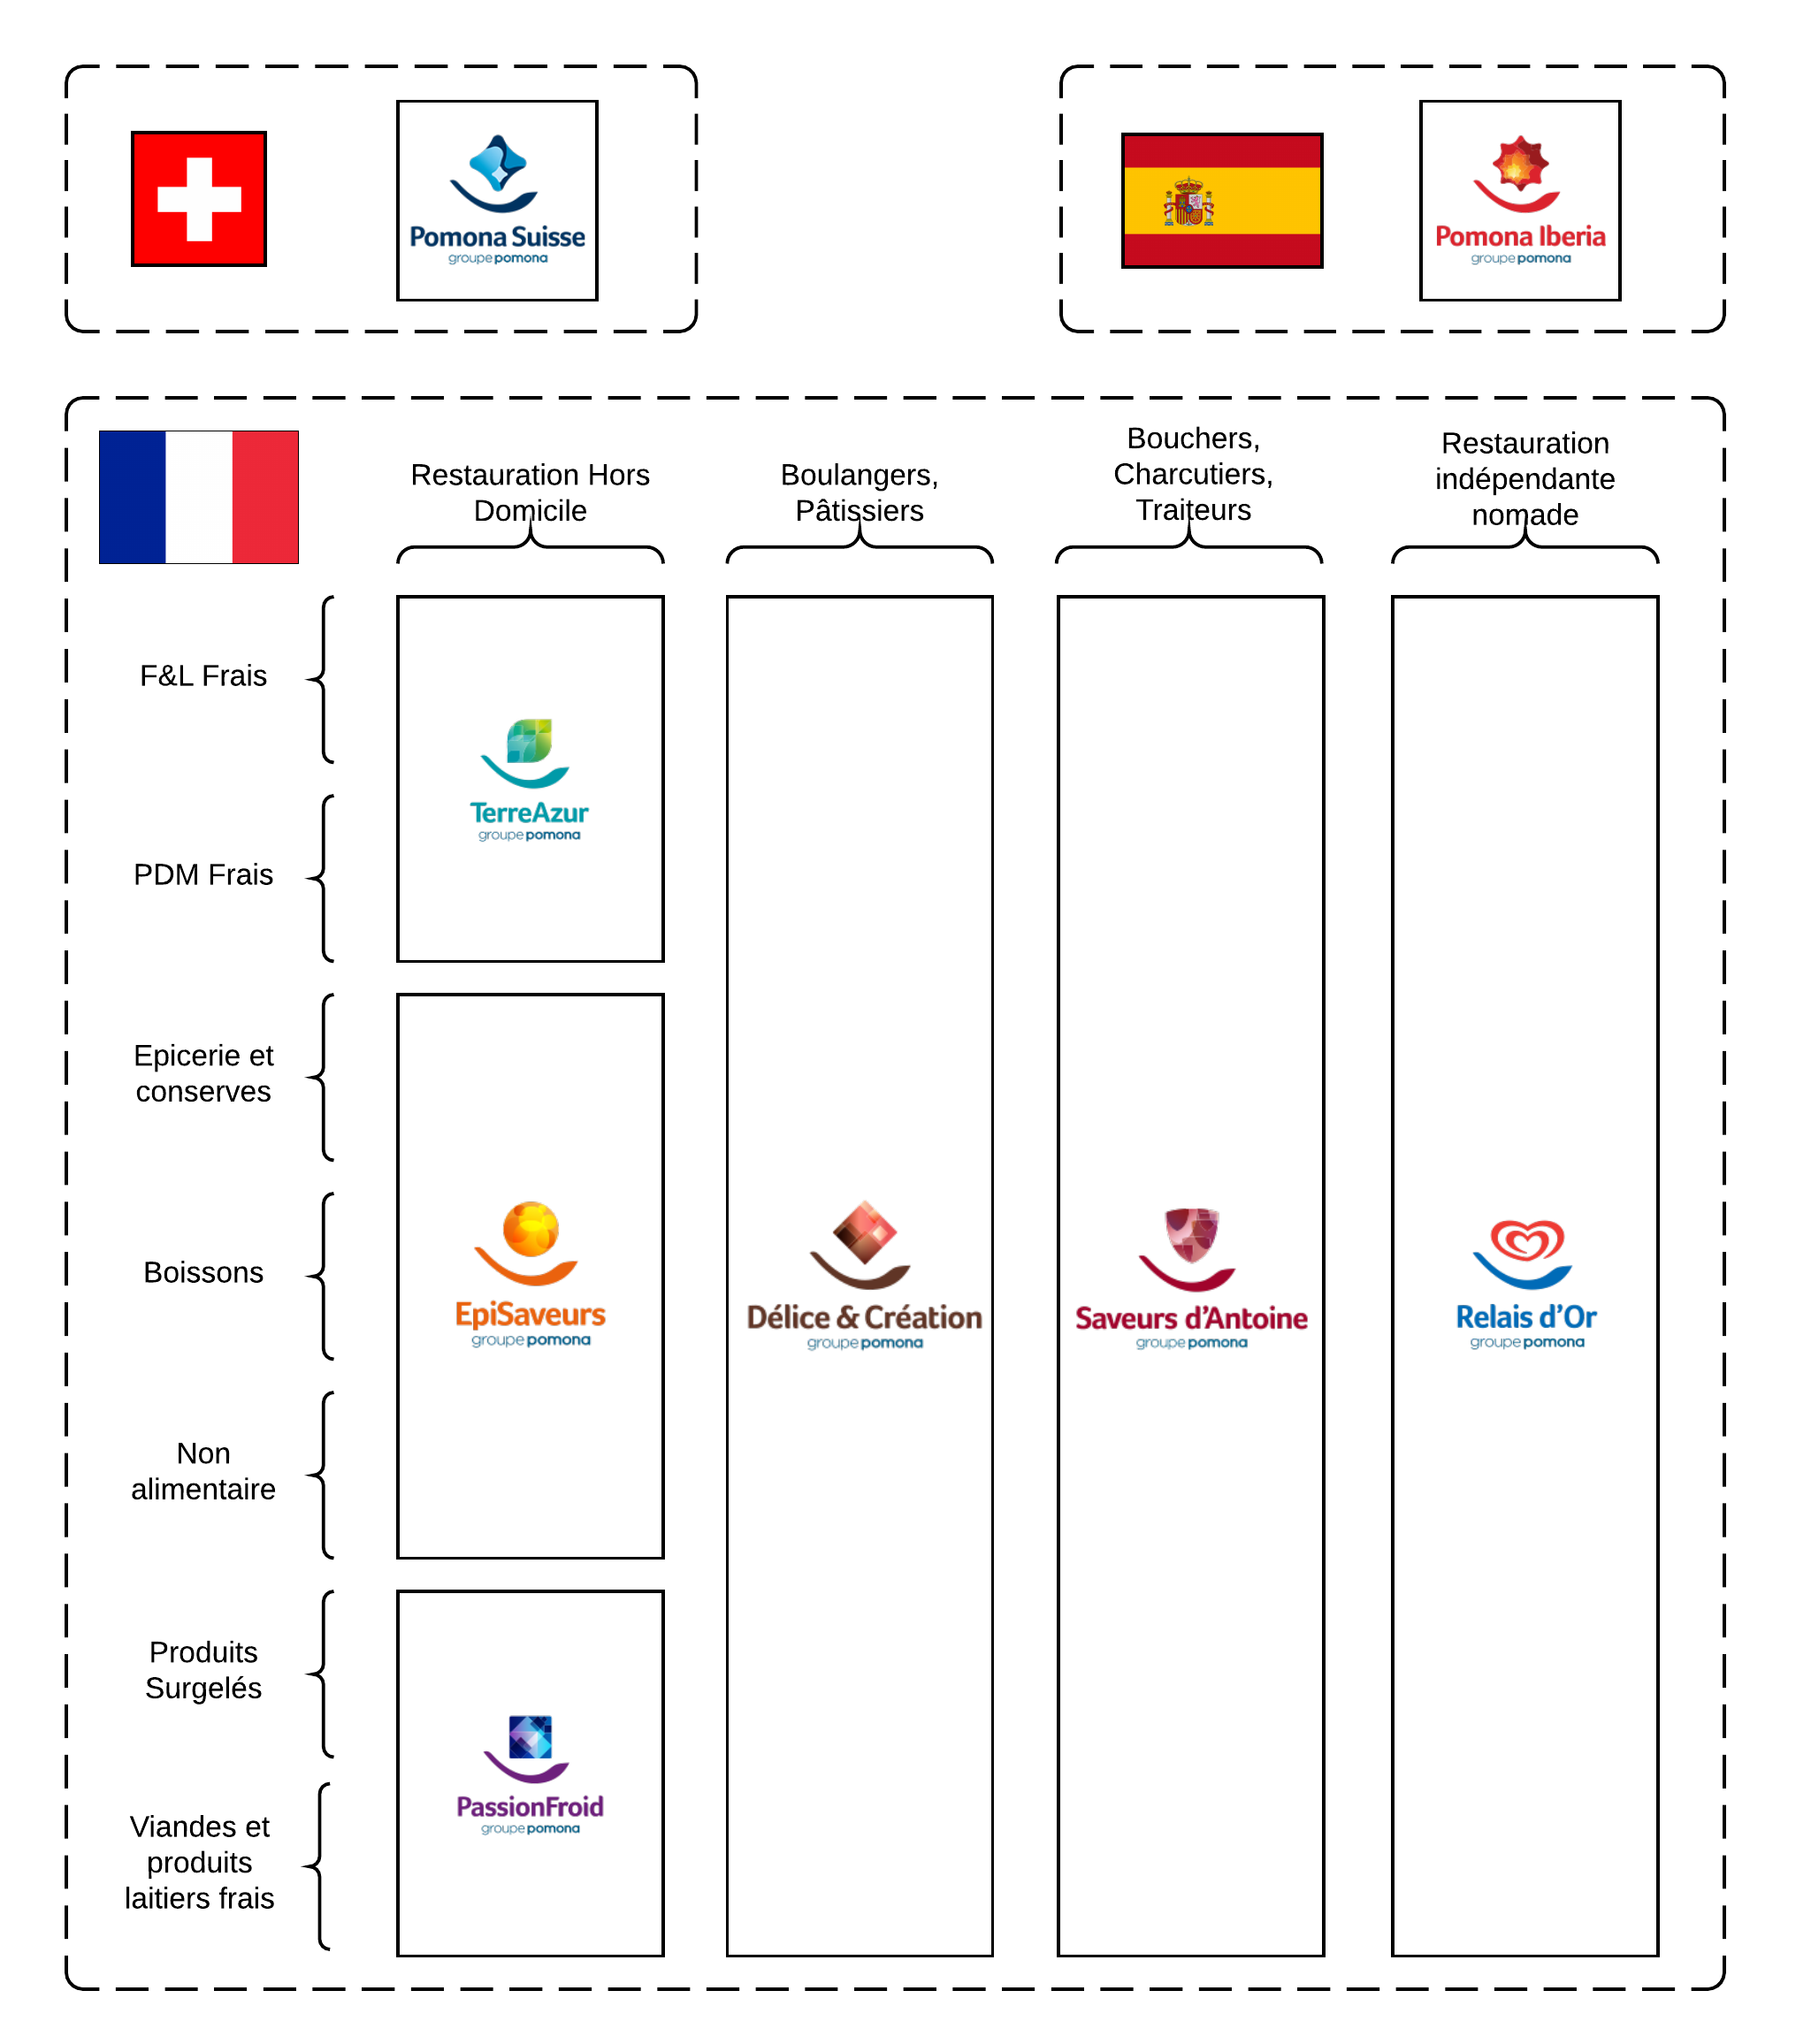
\includegraphics[width=\linewidth]{img/La repartition de lactivite des branches.png}
                    \end{center}
                    \caption{La répartition de l'activité des branches}
                    \label{fig:repartition_activite}
                \end{figure}

            \subsubsection{Le second niveau de décentralisation : les succursales}
            \label{les_succursales}
            Chacune des branches est elle-même à son tour décentralisée en un réseau d'entrepôts régionaux : les succursales (parfois également appelées simplement \og régions\fg).
            Ces succursales sont gérées comme des PME indépendantes, avec un directeur et un compte de résultat qui leur est propre.
            Si certaines négociations avec des fournisseurs ou des clients nationaux sont parfois menées par les branches, les succursales sont autonomes dans :
            \begin{itemize}
                \item{la définition de leur assortiment, même si des contraintes s'appliquent}
                \item{la stratégie de développement commercial}
                \item{la négociation des prix d'achat}
                \item{la négociation des prix de vente}
                \item{la politique de rémunération de leurs employés}
            \end{itemize}
            
            \`{A} ce titre, elles ont leurs propres équipes d'achat, leurs équipes commerciales (télévente et vente route), leurs équipes administratives et évidemment leurs équipes logistiques (essentiellement en entrepôt et les chauffeurs livreurs en charge des livraisons client).

            Certaines activités restent de la responsabilité des équipes centrales des branches, comme : la négociation avec les clients ou les fournisseurs nationaux, la constitution de l'assortiment commun (les produits que toutes les succursales doivent détenir), la gestion des référentiels de données de base métier, \dots
            
            Un exemple de maillage régional est présenté en \reffig{fig:reseau_es}, sachant que ce maillage régional est différent pour chacune des branches.
            \begin{figure}[htpb]
                \begin{center}
                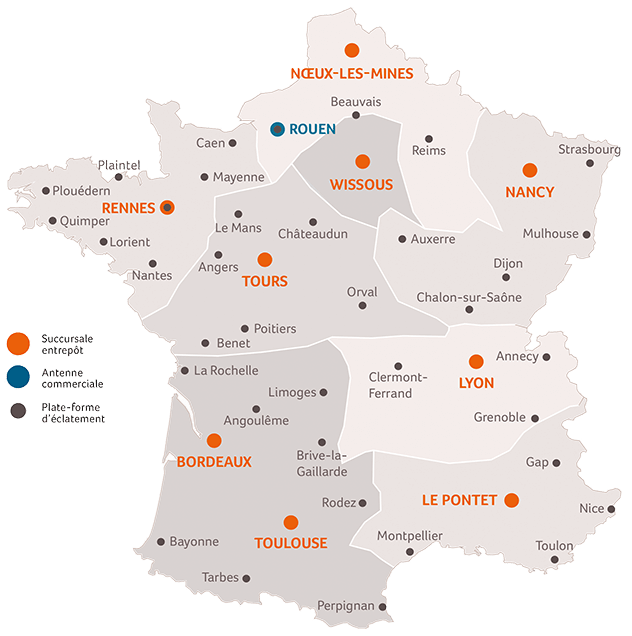
\includegraphics[width=\linewidth]{img/reseau es.png}
                \end{center}
                \caption{Le maillage régional de la branche \'{E}piSaveurs}
                \label{fig:reseau_es}
            \end{figure}


    \section{La gestion de l'information produit}
    
        \subsection{L'information produit}
        
            \subsubsection{Utilisations de l'information produit}
            \label{utilisation_info_produit}

                \paragraph{Conformité réglementaire}
                La gestion de l'information produit est essentiellement une contrainte réglementaire à statisfaire.
                Comme mentionné au préambule, la réglementation autour de l'information des consommateur s'est sans cesse complétée au cours des dernières années.
                Un des textes centraux est le règlement n°1169/2011 dit INCO (INformation COnsommateur)\cite{incotext}\cite{incoexpl}.
                C'est ce règlement qui définit l'ensemble des informations qui doivent être étiquetées sur le produit (liste d'ingrédients, tableau de données nutritionnelles, \dots), mais également affichée au client lors de commande en ligne sur les sites de e-commerce.
                Il s'agit principalement d'informations relatives à la sécurité alimentaire (ex : les allergènes) ou la santé (ex : informations nutritionnelles).

                \paragraph{Attentes client}

                Les consommateurs finaux (les \og convives \fg) étant de plus en plus sensibles au contenu de leur assiette, les clients du groupe sont de plus en plus demandeurs d'informations relatives aux produits qu'ils commandent.
                Ils demandent donc régulièrement des informations qui vont au-delà de ce qui est normalement prévu par la réglementaition.

                De plus, sur certains marchés pour lesquels des contrats courant sur de longues périodes - jusqu'à un an - sont établis (les marchés publics sont très concernés), il n'y a pas d'échantillonnage des produits.
                La seule manière pour ces clients d'évaluer la qualité des produits est de se référer aux documents contenant les informations produit, fournis par les distributeurs.

                \paragraph{Gestion}

                Certaines informations relatives aux produits sont nécessaires pour des raison de gestion adminsitrative.
                Par exemple, la gestion des taxes sur les produits alimentaires est complexe : 
                \begin{itemize}
                    \item les taux de TVA sont variables en fonction du type de produit
                    \item des taxes spécifiques s'appliquaient aux produits contenant de l'huile ou de la farine
                    \item des règlements particuliers s'appliquent aux alcools
                    \item \dots
                \end{itemize}
                D'autres informations, comme la nomenclature douanière, sont nécessaires pour effectuer les déclarations auprès des douanes européennes.

                Un autre type d'information capital pour la gestion des flux d'achat et de vente sont les informations logistiques, qui définissent par exemple le nombre d'unités consommateur dans le colis, le nombre de colis sur une palette, \dots
                Une gestion rigoureuse de ces informations est indispensable pour que les flux d'achat ou de vente soient correctement exécutés (que les quantités commandées soient les bonnes, que les montants facturés soient corrects, \dots).

            \subsubsection{Des produits bruts aux produits transformés}

            Le niveau d'exigence en termes d'information produit est variable en fonction du niveau de transformation de ce produit.
            Par exemple, sur des fruits et légumes frais, à peu de choses près seul le pays d'origine doit être affiché au client.
            Sur une barre chocolatée, ou un plat cuisiné, il sera nécessaire d'afficher :
            \begin{itemize}
                 \item une liste d'ingrédients (mettant en évidence les allergènes)
                 \item un tableau de données nutritionnelles (protéines, glucides, \dots)
                 \item une dénomination réglementaire
            \end{itemize}

            \subsubsection{Les grands types d'information}
            \label{info_produit}

            On se focalisera dans ce paragraphe sur les informations relatives aux \emph{produits alimentaires}.

                \paragraph{La composition}
                \label{composition}

                La première grande famille de données réglementaires sont les données de composition.
                Elles détaillent quels sont les ingrédients qui sont mis en oeuvre dans la fabrication des produits.
                \'{E}videmment, la composition a en général plus de sens pour les produits transformés que pour les produits bruts.
                Elle peut prendre la forme d'un texte listant la liste des ingrédients (l'étiquetage de ce texte est en général obligatoire sur les emballages des produits), ou d'un tableau.
                
                Les ingrédients incluent également les additifs.
                Il s'agit de substances ajoutées à la recette pour répondre à des fonctions particulières (colorant, exhausteur de goût, émulsifiant, \dots).
                Elles ne représentent en général qu'un pourcentage en masse négligeable dans la composition totale du produit.

                Le pourcentage en masse est parfois inclus sur certains ingrédients. 
                La règlementation l'oblige dans certains cas, par exemple quand l'ingrédient en question est mentionné dans la dénomination du produit (pour une \emph{tarte aux framboises}, la proportion de framboise doit être mentionnée dans la composition).

                Enfin, un aspect à la fois règlementaire et particulièrement important est la présence d'allergènes dans la composition.
                Le règlement INCO\cite{incotext}\cite{incoexpl} impose de mettre en évidence les allergènes relevant d'une des 14 catégories suivantes :
                \begin{enumerate}
                    \item Céréales contenant du gluten, à savoir blé, seigle, orge, avoine, épeautre, kamut ou leurs souches hybridées, et produits à base de ces céréales
                    \item Crustacés et produits à base de crustacés
                    \item \OE ufs et produits à base d’ \oe ufs
                    \item Poissons et produits à base de poissons
                    \item Arachides et produits à base d'arachides
                    \item Soja et produits à base de soja
                    \item Lait et produits à base de lait (y compris le lactose)
                    \item Fruits à coque, à savoir: amandes, noisettes, noix, noix de cajou, noix de pécan, noix du Brésil, pistaches, noix de Macadamia ou du Queensland, et produits à base de ces fruits
                    \item Céleri et produits à base de céleri
                    \item Moutarde et produits à base de moutarde
                    \item Graines de sésame et produits à base de graines de sésame
                    \item Anhydride sulfureux et sulfites
                    \item Lupin et produits à base de lupin
                    \item Mollusques et produits à base de mollusques
                \end{enumerate}
                Il peut y avoir deux niveaux de présence d'un allergène dans un produit (au-delà de la simple absence) :
                \begin{description}
                    \item[intentionnellement mis en oeuvre :] dans le cas où un ingrédient allergène fait volontairement partie de la recette. Ex : présence de moutarde dans un plat cuisiné.
                    \item[contamination croisée :] par exemple lorsque le produit fini est issu d'une chaîne de transformation qui traite un ingrédient allergène, mais que cet ingrédient ne fait pas partie de la recette. Ce cas de figure est en général mis en évidence par des mentions telles que \emph{"Peut contenir des traces de soja"} ou bien \emph{"Transformé dans un atelier processant également des fruits à coques et du sésame"}.
                \end{description}

                \paragraph{Les informations nutritionnelles}
                \label{donnees_nut}

                Une autre grande famille d'information produit sont les informations nutritionnelles. 
                Elles détaillent la quantité des principaux nutriments contenus dans les produits.
                Certains d'entre eux sont rendus obligatoires par le règlement INCO~\cite{incotext}\cite{incoexpl} cf. l'exemple de tableau à la \reftable{tab:donnees_nut}, et d'autres sont optionnels, comme par exemple la quantité de fer, de calcium, \dots

                \begin{table}[htbp]
                    \begin{center}
                    \begin{tabularx}{\linewidth}{|X|X|X|X|}
                        \hline
                        \textbf{Informations nutritionnelles} & \textbf{Pour 100g} & \textbf{Pour un biscuit} & \textbf{\% des AJR pour un biscuit} \\
                        \hline
                        \'{E}nergie &1674 kJ
                        
                        398 kcal & 209 kJ
                        
                        50 kcal & 3 \% \\
                        \hline
                        Protéines & 3.0 g & 1.0 g & 3 \% \\ 
                        \hline
                        Matières grasses & 13.0 g & 1.6 g & 2 \% \\
                        \hline
                        dont acides gras saturés & 5.8 g & 0.7 g & 4 \% \\
                        \hline
                        Glucides & 66 g & 8.2 g & 3 \% \\
                        \hline
                        dont sucres & 48 g & 6.1 g & 7 \% \\
                        \hline
                        Fibres alimentaires & 2.5 g & 0.3 g &\\
                        \hline
                        Protéines & 3.3 g & 0.4 g & 1 \% \\
                        \hline
                        Sel & 0.41 g & 0.05 g & 1 \% \\
                        \hline
                    \end{tabularx}
                    \end{center}
                    \caption{Exemple de tableau de données nutritionnelles}
                    \label{tab:donnees_nut}
                \end{table}
                La réglementation rend obligatoire de mentionner les informations nutitionnelles de cette table pour 100g, ou 100mL de produit (pour les boissons).

                Les informations nutritionnelles peuvent également se présenter sous forme d'allégations, qui ont des définitions précises dans la réglementation. Ces allégations peuvent être : \emph{sans sel, faible en sucres, riche en fibres, \dots}

                \paragraph{Les origines}

                Du fait de la complexification des opérations de transformation et de la complexification des flux d'échanges de marchandises, l'origine des produits alimentaires est une notion qui n'est pas définie avec précision dans l'absolu.
                Il n'y a donc pas non plus de réglementation précise sur le sujet, si ce n'est que l'information produit doit toujours être présentée de manière loyale au consommateur.
                On peut se donner une règle simple pour définir l'origine d'un produit alimentaire: plus il est brut, plus va compter l'origine de ses ingrédients ; plus il est transformé, plus va compter le lieu de dernière transformation.

                Par exemple, sur des morceaux piécés de viande fraîche, on aura des origines multiples en fonction du pays de naissance, d'élevage ou d'abattage de la bête.
                Et à l'inverse, sur un steak haché cette information n'aura aucun sens dans la mesure où il est produit d'un assemblage de \og minerais \fg pouvant provenir de multiples pays.
                L'industriel pourra choisir de communiquer sur le fait que la viande a été transformée en steak dans telle usine par exemple.

                \paragraph{Les données logistiques} 

                On appelle données logistiques essentiellement le plan de palettisation et de conditionnement du produit.
                Il s'agit de la définition de la \og hiérarchie logistique \fg du produit.
                Cette hiérarchie se base d'abord sur la définition d'une \og unité de base \fg qui est la plus petite unité légalement détaillable (i.e. qui porte l'ensemble des informations réglementaire pour sa commercialisation).
                Ces notions ont été standardisées par l'organisme international de standardisation GS1\cite{GDSNimplementationGuide}.
                Deux exemples pour illustrer : 
                \begin{itemize}
                    \item pour un boîte de sachets de thé, l'unité de base est la boite car les sachets de thé ne portent pas les informations nécessaires à leur commercialisation
                    \item pour un paquet de barres chocolatées (comme celles qu'on peut trouver au détail en boulangerie), l'unité de base est la barre car elle porte l'ensemble des mentions réglementaires sur son emballage
                \end{itemize}
                La hiérarchie logistique est à la fois :
                \begin{itemize}
                    \item la définition des niveaux successifs d'emballage des produits  : combien d'unités de base dans un paquet, combien de paquets dans un carton, combien de cartons sur une palette, \dots
                    \item la définition du contenu de l'unité de base (ex : le nombre de sachets de thé, le nombre de doses dans une boîte d'aides culinaires, \dots)
                \end{itemize}

                Les données logistiques concernent également les durées de vie du produit (qu'il s'agisse de Date Limite de Consommation ou Date de Durabilité Minimale) :
                \begin{itemize}
                    \item la durée de vie totale à fin de production
                    \item la durée de vie garantie à la livraison
                \end{itemize}
                
                Parfois, certaines contraintes d'approvisionnement peuvent être mentionnées : 
                \begin{itemize}
                    \item unités commandables (ex : on ne peut commander que des cartons complets)
                    \item multiples de commande (ex : on ne peut commander les cartons que 10 par 10 pour des raisons de montage des palettes)
                    \item minimum de commande (ex : il faut commander au minimum 30 cartons)
                \end{itemize}
                mais elles sont dépendantes d'un accord entre l'industriel et son client distributeur et ne sont donc pas à proprement parler des informations produit.

                \paragraph{Les données administratives et financières}

                Les données dites administratives et financières regroupent le reste des informations de gestion pour lesquelles il existe des contraintes réglementaires.
                Il s'agit :
                \begin{itemize}
                    \item du taux de TVA du produit
                    \item de sa nomenclature douanière et du pays d'origine au sens de la déclaration d'échange de biens\cite{notions_DEB}
                    \item de toute autre taxe applicable au produit
                \end{itemize}

                \paragraph{Les labels} 
                \label{labels}

                Afin de garantir des qualités spécifiques à certains produit, des organismes de certification ont mis en place des labels pouvant s'appliquer aux produits.
                En général, ils se basent sur des cahiers des charges et peuvent être assortis d'audits de certification ou de contrôle.
                Ils peuvent garantir des méthodes de production ou transformation, des lieux de production, des caractéristiques de leurs ingrédients, des pratiques commerciales équitables, \dots
                Les types de labels les plus connus sont :
                \begin{itemize}
                    \item les produits Biologiques
                    \item les origines protégées (Appellation d'Origine Protégée, Indication Géographique Protégée, \emph{viandes} de France, Bleu Blanc Cor, Régions UltraPériphériques d'Europe\dots)
                    \item les pratiques commerciales équitables (Max Havelaar, \dots)
                    \item les modes de production respectueux de l'environnement (Aquaculture Stewardship Council, Marine Stewardship Council, Roundtable on Sustainable Palm Oil, Nordic Swan, \dots)
                    \item la qualité \og générale \fg des produits (Label Rouge, \dots)
                \end{itemize}

                \paragraph{Les données marketing}

                Certaines données marketing font également partie de l'information produit.
                La plus évidente est la marque commerciale du produit, qui parfois définit totalement le produit.
                Par exemple, on sait ce qu'est un Snickers, de la Mousline, du Nutella, \dots
                Les produits peuvent également porter d'autres allégations marketing, non réglementaires ou labelisantes : \'{E}lu produit de l'année, Vu à la télé, Issu de notre savoir-faire centenaire, \dots                

        \subsection{Le processus}
        
            \subsubsection{Le fournisseur est propriétaire des informations produit}

            Comme présenté à la section \mref{business}, le Groupe Pomona n'a pas d'activité de fabrication ou de transformation de marchandises.
            \`{A} ce titre, l'ensemble des données produits ne peuvent être déterminées que par les fournisseurs de ces produits.
            L'ensemble des entités du groupe s'appuient donc sur les données transmises par les industriels ou producteurs de marchandises.

            Il peut arriver que certains produits soient achetés par Pomona à d'autres négociants non-producteurs.
            Dans ce cas, de la même manière que le groupe Pomona a la responsabilité de collecter puis transmettre les informations produit à ses clients, ces fournisseurs négociants doivent eux-même aller chercher l'information produit et la transmettre à Pomona.

            \emphbox{Dans tous les cas, c'est le \emph{fournisseur} qui est responsable de produire et de transmettre l'information produit aux entités du groupe Pomona.}

            \subsubsection{La notion de produit et d'article}
            \label{produit_article}

            Un mot sur la modélisation des données adoptée est nécessaire pour comprendre les grandes lignes du processus.
            Comme il a été vu à la section \mref{les_branches}, certains produits sont susceptibles d'être commercialisés par plusieurs branches du groupe.
            
            De plus, du fait que les systèmes d'information ne sont pas identiques entre les branches, certaines contraintes imposent parfois des différences de modélisation, des duplications volontaires de codes pour répondre à ces contraintes.
            Une illustration de ce point pour clarifier : la facturation client pour une canette de soda peut se faire au litre (permet de comparer les prix entre les différents conditionnement et les différentes marques) ou à la cannette (permet de se faire une idée du coût portion d'un produit).
            Or, la possibilité de pouvoir facturer un même article dans plusieurs unités différentes n'est pas une fonctionnalité offerte par tous les systèmes d'information.
            En particulier, \'{E}piSaveurs peut gérer dans ce cas un unique article et le facturer dans l'unité de son choix en fonction des demandes des clients.
            Mais Délice et Création (qui possède un système d'information différent) doit dupliquer cet article car une seule unité de facturation est possible pour un article donné.

            Enfin, au-delà des contraintes liées au SI, certaines pratiques imposent de laisser aux branche une indépendance forte dans la gestion de leurs référentiels articles.
            Il faut savoir que commercialiser sous un même code article des produits qui sont similaires permet d'obtenir des gains de productivité à plusieurs niveaux :
            \begin{itemize}
                \item on économise des emplacements en entrepôt (un emplacement ne peut contenir qu'un article)
                \item on gagne du temps administratif dans la gestion des prix : le foisonnement d'articles impose de gérer plus de prix client
                \item \dots
            \end{itemize}
            La contrepartie à adopter cette pratique est qu'il n'est alors plus possible de différencier ces produits similaires, par exemple pour leur appliquer des prix de vente distincts, ou bien offrir la possibilité à un vendeur de garantir au client la livraison d'un produit plutôt que l'autre.
            Néanmoins, en fonction de la clientèle adressée, certains produits pourront être considérés comme similaires, alors que pour d'autres ils ne seront pas interchangeables.
            Cet exemple est détaillé dans la \reffig{fig:produit_article}.

            On différencie donc les deux notions suivantes : 
            \begin{description}
                \item[les produits :] ils représentent une marchandise physique produite par un fournisseur. Ce sont les produits qui portent les \emph{informations produit} décrites à la section \mref{info_produit}. Un produit ne peut appartenir qu'à un seul fournisseur. Le référentiel produit est unique pour l'ensemble du groupe.
                \item[les articles :] ce sont les objets qui sont gérés par les branches dans leurs systèmes de gestion respectifs. Leurs attributs sont très liés au système d'information qui les porte. Chaque branche gère de manière autonome son référentiel article, incluant les liens qui sont faits entre produits et articles.
            \end{description}
            Cette modélisation permet de répondre à l'ensemble des contraintes présentées dans ce paragraphe.

            \begin{figure}[htbp]
                \begin{center}
                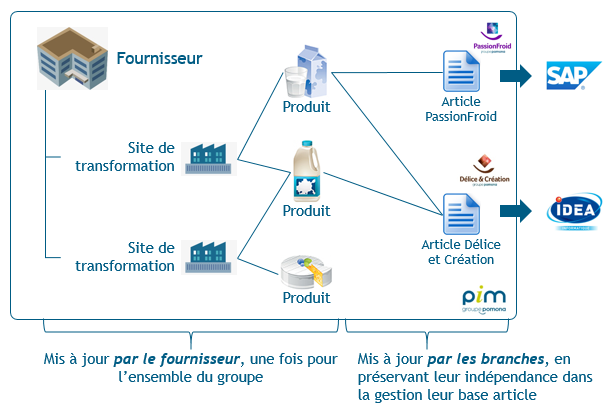
\includegraphics[width=0.8\linewidth]{img/Produit article.png}
                \end{center}
                Dans cet exemple fictif, le type de conditionnement du lait n'a aucun impact sur les clients de la branche Délice et Création. Elle commercialise donc sous un même code article deux produits distincts.

                Pour des raisons de contrainte de conservation, la branche PassionFroid a quant à elle choisi de ne commercialiser qu'un seul produit - en brique. Elle pourrait choisir d'ouvrir un nouveau code article pour le lait en bouteille (non représenté sur le schéma ci-dessus).
                \caption{La distinction entre produit et article}
                \label{fig:produit_article}
            \end{figure}          

            \subsubsection{Les acteurs}

                \paragraph{L'acheteur}
                L'acheteur peut être en succursale, ou à la centrale d'achat de la branche (cf. \mref{les_branches} et \mref{les_succursales}).
                Il est responsable de l'assortiment, i.e. des articles qui sont commercialisé par sa branche, ou sa succursale.
                Il est à l'origine de la création d'un nouveau produit, dans la mesure où c'est lui qui va décider de le référencer ou pas.
                La gestion de l'information produit ne représente qu'une petite partie de l'ensemble de ses responsabilités (qui peuvent inclure négociations fournisseurs, gestion du sourcing, gestion des approvisionnements, prévisions d'évolution des prix, \dots).

                \paragraph{Le fournisseur}
                Il a été vu que le Groupe Pomona - dans sa qualité de distributeur - n'est pas en mesure de déterminer seul les informations produit sur les marchandises qu'il commercialise.
                \`{A} ce titre, les équipes des fournisseurs sont en charge de transmettre les information produit à Pomona.
                En général, ce sont deux types de profil qui effectuent cette tâche : 
                \begin{itemize}
                    \item les commerciaux (aux sens large, incluant les assistants commerciaux)
                    \item les ingénieurs qualité
                \end{itemize}

                \paragraph{Le gestionnaire de référentiel - SEGER}
                Le gestionnaire de référentiel travail au SErvice de GEstion des Référentiels (SEGER), qui sont des équipes positionnées au niveau des branches (cf. \mref{les_branches}).
                Ils sont responsables de la qualité des données dans les référentiels métier (articles, fournisseurs, clients, \dots).
                La gestion des données de base dans les référentiels est leur mision principale.

                \paragraph{L'ingénieur qualité}
                L'ingénieur qualité travaille à la DQSE ou en succursale (cf. \mref{les_directions_fonctionnelles} et \mref{les_succursales}).
                Dans le processus de gestion de l'information produit, il est en charge de contrôler la qualité des données, mais également leur conformité réglementaire (ex : on ne peut qualifier un produit de \og faible en sel \fg que s'il comporte moins de n grammes de sel pour 100 grammes de produit.)
                La gestion de l'information produit ne représente qu'une partie des responsabilités de l'ingénieur qualité.

            \subsubsection{Les contrôles}
            \label{controles}
            Comme cela a été vu dans la section \mref{utilisation_info_produit}, il est nécessaire que les différentes entités du groupe soient en possession d'une information produit fiable.
            Or, avoir des données de qualité nécessite des efforts de la part des métiers, en particulier lorsque le processus n'est pas entièrement porté en interne dans la société.
            \`{A} ce titre, plusieurs étapes de contrôle ont été définies dans le processus de gestion du référentiel de données produit et article :
            \begin{description}
                \item[lorsque le fournisseur a saisi les données produit :] la personne à l'origine de la demande de référencement (en général, un acheteur) doit contrôler la cohérence des données produit
                \item[lorsque le demandeur a demandé la création d'un article :]  le gestionnaire de référentiel valide à nouveau la cohérence des informations produit
                \item[après la création article, de manière asynchrone :] le service qualité contrôle par échantillonnage les données d'une partie des produits et articles qui ont été modifiés pendant une période.
            \end{description}
            Le retour d'expérience montre que ces contrôles, loin d'être redondants, sont nécessaires pour avoir une qualité de données acceptable.
            Ces processus de contrôle sont décrits à la \reffig{fig:processus_article}.

            \begin{figure}[htpb]
                \begin{center}
                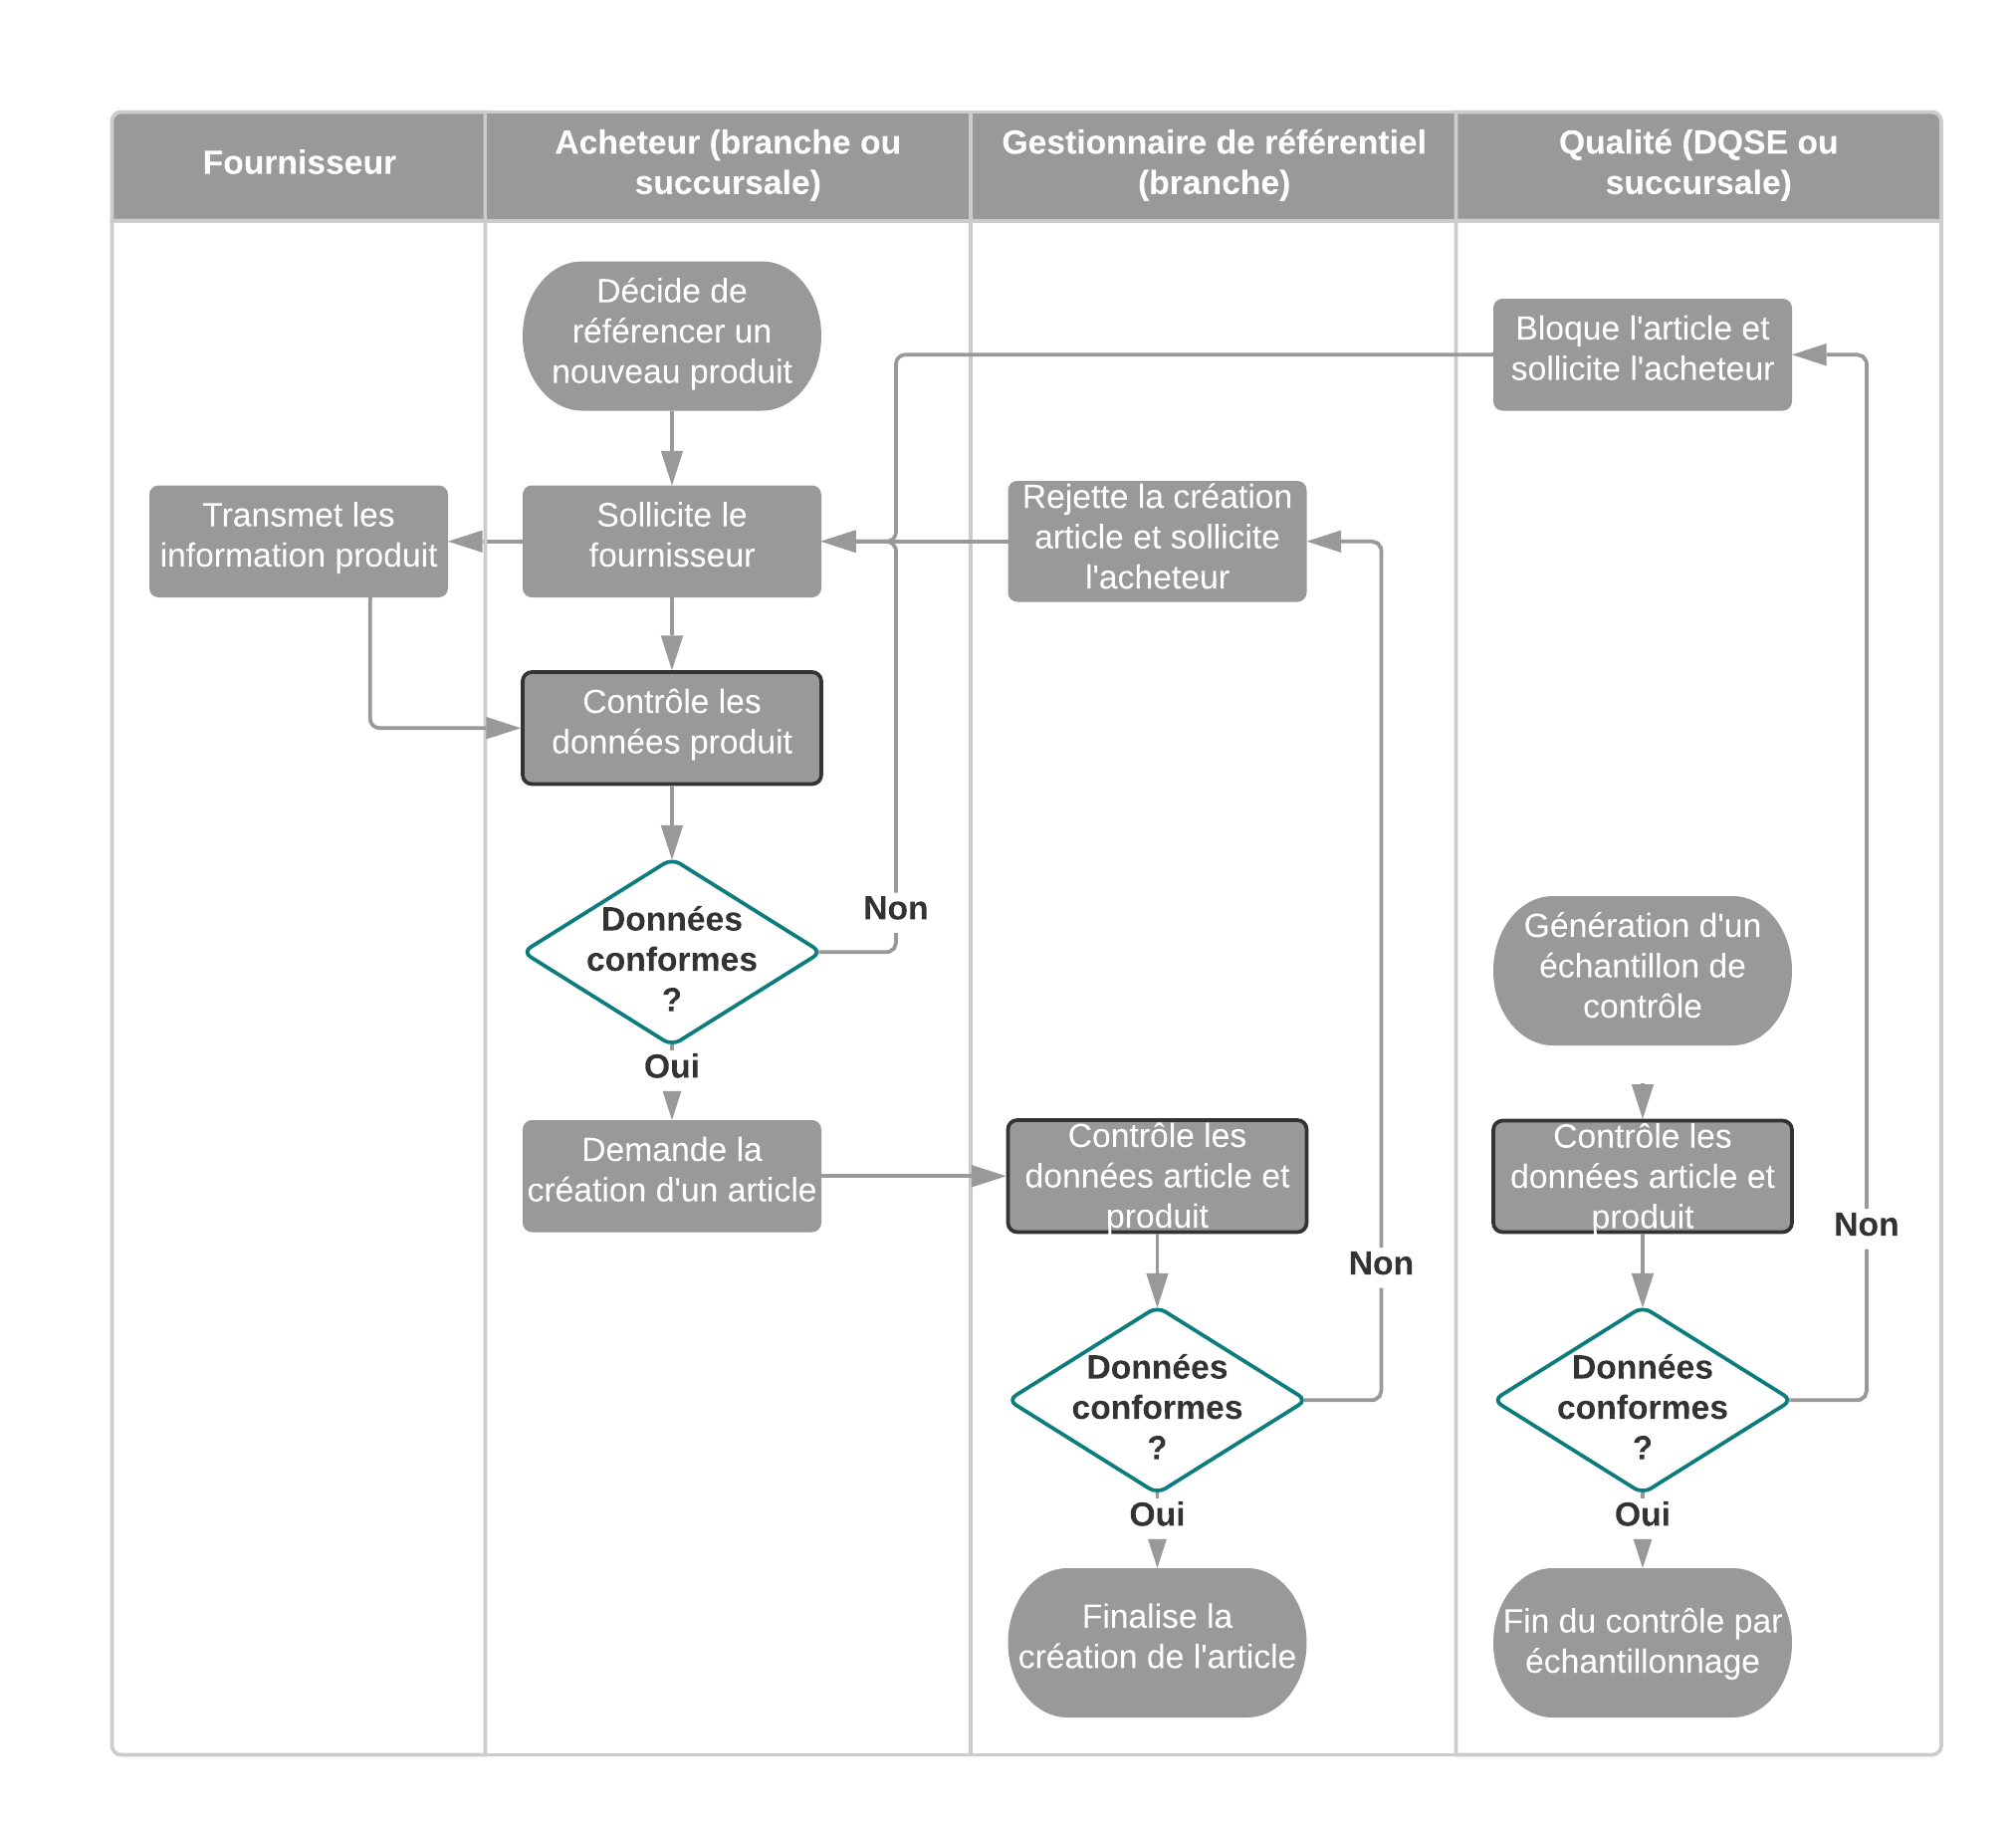
\includegraphics[width=\linewidth]{img/Processus de creation article.png}
                \end{center}
                \caption{Le processus de création article}
                \label{fig:processus_article}
            \end{figure}    

            Les contrôles effectués à chacune des étapes sont les suivants : 
            \begin{description}
                \item[contrôle de la complétude des données :] vérification que les données transmises comportent l'ensemble des données attendues
                \item[contrôle de cohérence entre les données :] vérification que les informations transmises sont cohérentes entre elles (ex : un allergène présent dans la liste d'ingrédients du produit a bien été signalé comme allergène par ailleurs)
                \item[contrôle de la cohérence avec les pièces jointes :] en plus de données structurées, les fournisseurs transmettent également des fichiers portant des informations produit (ex : l'étiquette produit ou le visuel de l'emballage). Ces pièces jointes sont décrites à la section \mref{pieces_jointes}. La personne en charge du contrôle vérifie que les données transmises sont cohérentes avec ces documents.
            \end{description}

        \subsection{Les outils informatiques associés}
        \label{outils_infos}

        Comme vu dans la description des branches du groupe (voir section \mref{les_branches}), les outils informatiques ne sont pas tous les mêmes sur l'ensemble des branches.
        Ainsi, les outils utilisés pour la gestion de l'information produit ne sont pas les mêmes.

            \subsubsection{Les branches faiblement outillées}
            
            Les branches étrangères (Pomona Suisse, Pomona Iberia), spécialistes (Délice et Création, Saveurs d'Antoine) et la branche TerreAzur sont aujourd'hui faiblement outillées.
            Cela signifie que l'information produit est en général stockée uniquement sous la forme de fichiers (essentiellement les pièces jointes, décrites à la section \mref{pieces_jointes}).
            L'ensemble des échanges avec les fournisseurs se font par mail, et les articles sont créés directement dans les systèmes de gestion par les gestionnaires de référentiel.
            Les liens entre les articles et les informations produit ne sont pas matérialisés dans les systèmes informatiques.

            \subsubsection{Le GIP}
            \label{GIP}

            Le GIP (Gestion de l'Information Produit) est utilisé sur la branche PassionFroid.
            C'est un système de gestion de l'information produit qui est maintenant obsolescent et en cours de remplacement.
            Il a toutefois le mérite de permettre le stockage dans une application des données et des pièces jointes relatives aux produits, avec la possibilité d'accéder aux informations produit à partir des identifiants des articles.
            C'est ce système qui a permis de pouvoir alimenter les sites de e-commerce PassionFroid et \'{E}piSaveurs avec les informations produit.
            Il est toutefois ancien, et ne propose pas de fonctionnalité d'export en masse fiable.
            Il s'agit d'une application qui n'est pas ouverte aux utilisateurs externes au groupe, et les échanges avec les fournisseurs passent donc par des échanges de mails.

            \subsubsection{Le PIM}
            \label{PIM}

            Le PIM (Product Information Management) est un système de gestion de l'information produit qui a été mis en production en mai 2019, pour la branche \'{E}piSaveurs.
            Il a vocation a être déployé sur l'ensemble des branches du groupe.
            En terme de responsabilités, il vise à gérer la totalité des informations produit, mais également d'être maître sur les référentiels articles.
            Ce sera le système de référence pour tous les autres systèmes consommant de l'information produit, ou des données article.

                \paragraph{Description générale de l'outil}

                C'est un système qui porte l'ensemble du processus de gestion de l'information produit, tel que décrit à la \reffig{fig:processus_article}.
                Il est accessible aux fournisseurs du groupe, qui viennent directement mettre à disposition les données et les pièces jointes.
                Les fonctionnalités caractéristiques de ce système par rapport à d'autres systèmes informatiques sont :
                \begin{itemize}
                    \item la gestion de workflows (processus), qui permet d'orchestrer l'activité de l'ensemble des acteurs du système
                    \item la possibilité de paramétrer un modèle de données relativement complet, avec des centaines de métadonnées sur les différents objets
                    \item la présentation de l'interface utilisateur via le navigateur, qui permet de s'adresser simplement à des acteurs hors du groupe (pas de client lourd à installer)
                    \item la gestion performante de pièces jointes (documents informatiques) en grandes quantité
                    \item Une gestion de versions des objets robuste, permettant d'auditer l'historique ou de restaurer des données dans un état précédent
                \end{itemize}
                Cet outil porte entre autres les fonctionnalités de contrôle des informations, comme illustré à la \reffig{fig:ecran_PIM}.
                L'intégration du PIM au sein des systèmes informatiques du Groupe Pomona est décrite dans la \reffig{fig:integration_PIM}.

                \begin{figure}[htpb]
                    \begin{center}
                    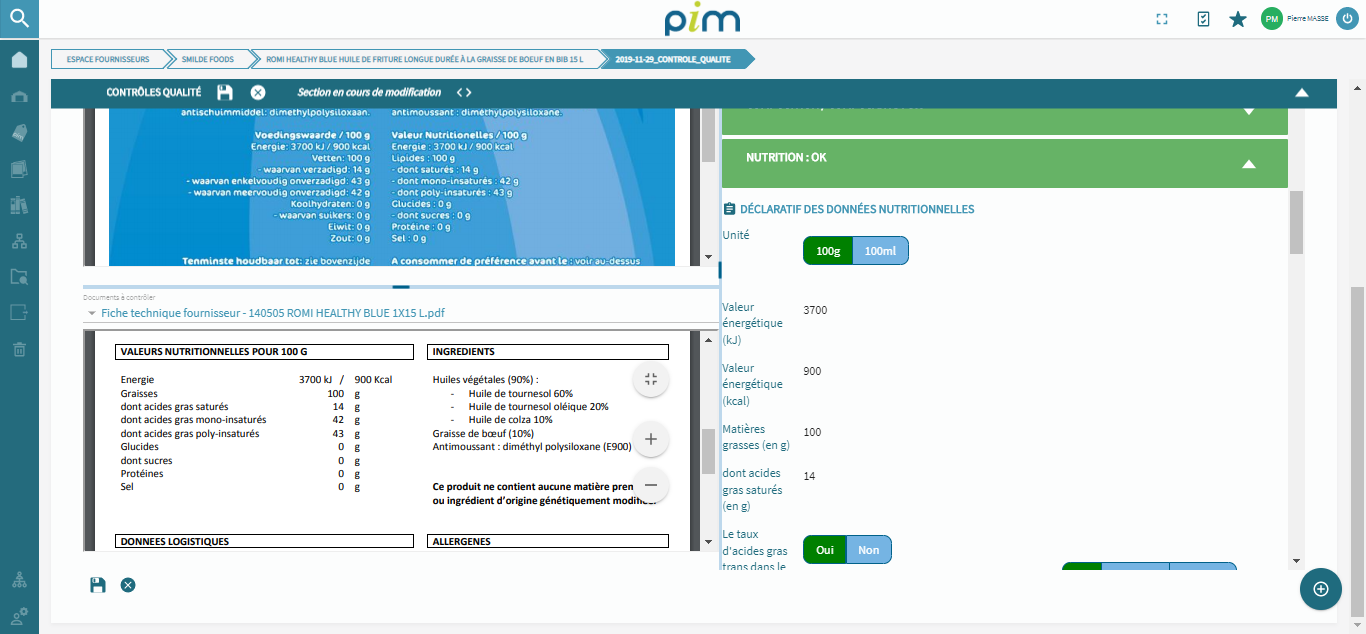
\includegraphics[width=\linewidth]{img/Ecran PIM.png}
                    \end{center}
                    Cette capture d'écran montre l'outil de contrôle des données produit. Sur la partie gauche, le contenu des pièces jointes est affiché (visuel de l'emballage en haut, fiche technique en bas), sur la droite les données qui ont été transmises par le fournisseur.
                    \caption{Une capture d'écran du PIM}
                    \label{fig:ecran_PIM}
                \end{figure} 

                \begin{figure}[htpb]
                    \begin{center}
                    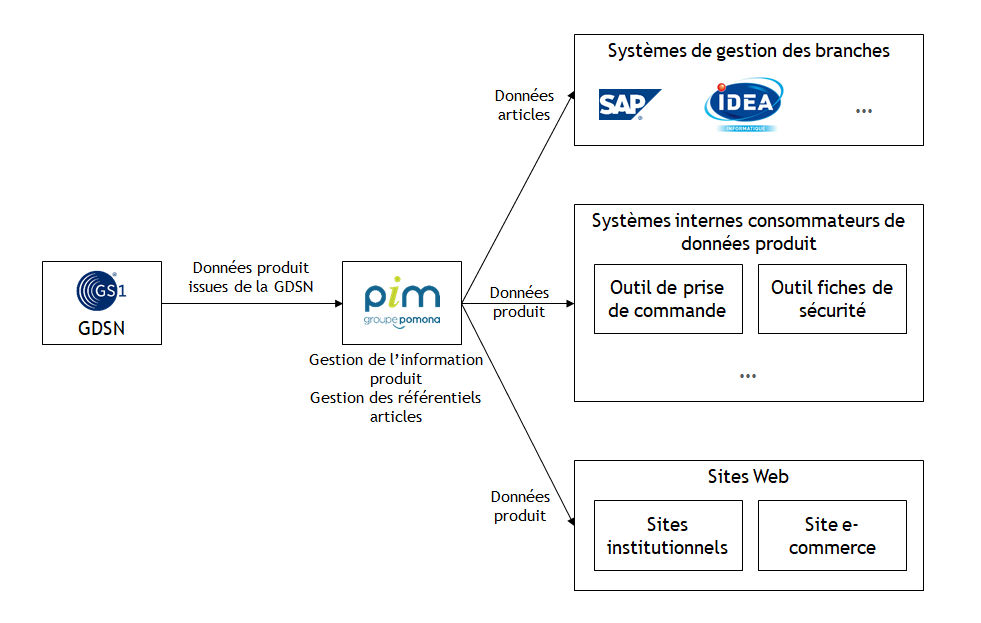
\includegraphics[width=\linewidth]{img/PIM_integration.png}
                    \end{center}
                    \caption{L'intégration du PIM au sein des systèmes du Groupe Pomona}
                    \label{fig:integration_PIM}
                \end{figure}

                \paragraph{Le socle technologique (et un mot de vocabulaire)}

                Ce logiciel a été construit sur la base de l'outil de gestion de contenu généraliste Nuxeo.
                Il s'agit d'un outil de GED (Gestion \'{E}lectronique de Documents), et tous les objets (produits, fournisseurs, articles, \dots) qu'il stocke sont nommés \og documents \fg.
                Dans le cadre du PIM, ce qui est habituellement appelé \og document \fg au sens d'un fichier informatique (document pdf, image png, vidéo, \dots) est appelé \og pièce jointe \fg.
                On utilisera ce vocabulaire dans le présent rapport.

                Le logiciel Nuxeo est adapté par une société - Keendoo - qui pré-paramètre la solution généraliste Nuxeo pour en faire un outil spécialisé dans la gestion d'information pour les produits alimentaires.

                La dernière \og couche \fg de développement a été réalisé de manière spécifique par les équipes de développement du Groupe Pomona.

                La base de données sous-jacente à l'application est une base NoSQL MongoDB.
 
                \paragraph{La GDSN}

                \label{GDSN}
                La GDSN (Global Data Synchronization Network) est un réseau d'échange de données produit entre industriels, distributeurs, restaurateurs, \dots
                Ce réseau est exploité par des opérateurs privés, mais le format et la chorégraphie des échanges ont été standardisés par l'organisme de standardisation GS1.
                Son schéma de principe est décrit à la \reffig{fig:GDSN}.
                Sans rentrer dans le détail, au sein du Groupe Pomona l'utilisation qui en est faite est de récupérer les informations depuis ce réseau d'échange, afin de préalimenter les données produit pour les fournisseurs.
                Cette foncitonnalité permet de faire gagner du temps aux fournisseurs pour leur éviter une partie de ressaisie, mais également de limiter les erreurs.
                Toutefois, cette fonctionnalité ne permet pas à elle seule de garantir une parfaite qualité de données.
                Il s'agit uniquement d'un \og tuyau \fg, si les données en entrée ne sont pas correctes, elles ne seront pas correctes en sortie.
                Pour aller plus loin dans la compréhension de ce réseau, il est possible de consulter les ressources mises en ligne par GS1~\cite{GDSN_GS1_FR}\cite{GDSN_GS1_GLOBAL}.

                \begin{figure}[htpb]
                    \begin{center}
                    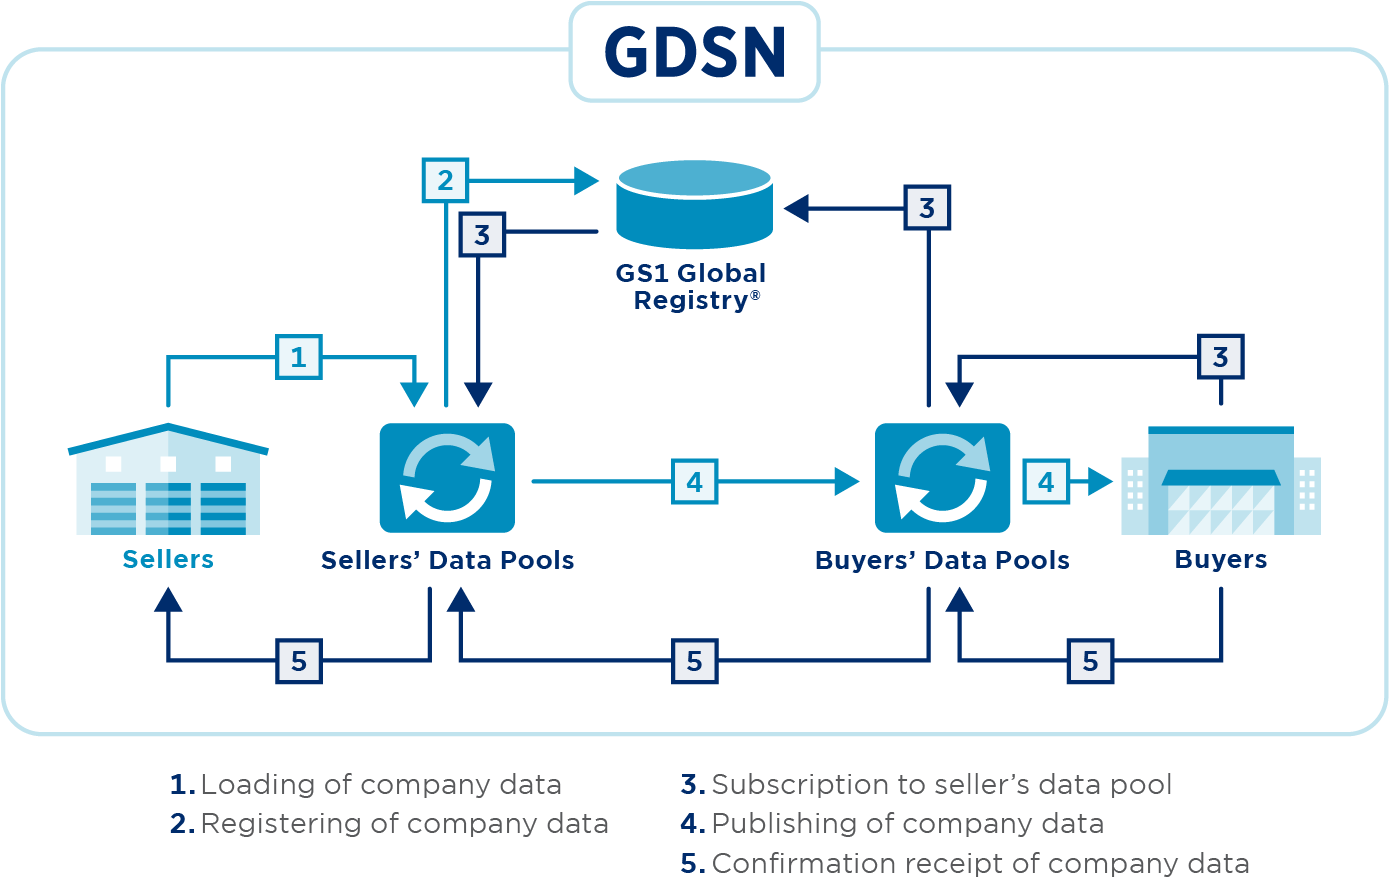
\includegraphics[width=\linewidth]{img/gdsn-schema.png}
                    \end{center}
                    \caption{Schéma de principe de la GDSN}
                    \label{fig:GDSN}
                \end{figure}                 
                
                \paragraph{L'identification des objets dans le PIM}
                \label{uid}

                Un dernier point à connaître à propos du PIM, est la manière d'identifier l'ensemble des objets en son sein.
                Chaque objet géré (ainsi que toute version archivée) porte un identifiant unique, nommé \emph{uid} qui est totalement univoque.
                Pour la suite, on se basera sur ces uid pour faire référence à des produits stockés dans le PIM.
                Une illustration est présentée à la \reffig{fig:uid}.

                \begin{figure}[htpb]
                    \begin{center}
                    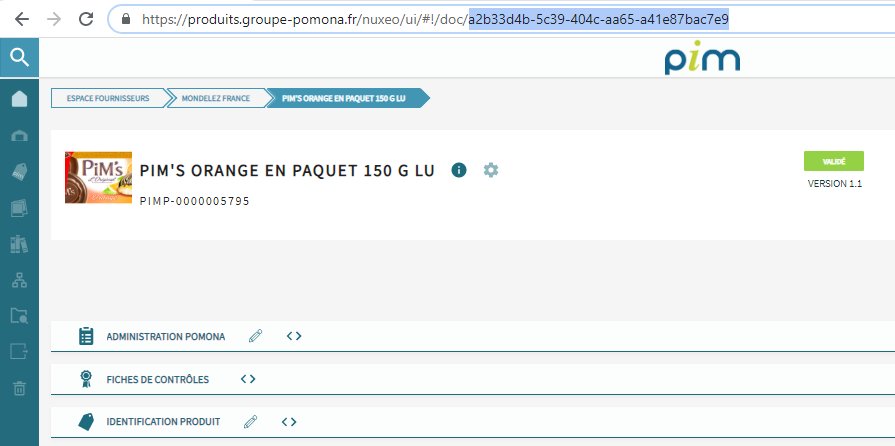
\includegraphics[width=\linewidth]{img/uid.png}
                    \end{center}
                    L'uid du produit affiché est mis en évidence dans l'url
                    \caption{L'uid d'un produit}
                    \label{fig:uid}
                \end{figure}                 

                \paragraph{Les API}

                Un des aspects intéressants du PIM pour l'exploitation en masse des données produit, est qu'il expose des API permettant d'aller requéter l'ensemble de son contenu.
                Cela concerne à la fois les données dites structurées, mais également les pièces jointes.
                Cela rend les données produit de la branche \'{E}piSaveurs bien plus simplement accessibles que celles des autres branches.

                \paragraph{La reprise de données initiale et la migration}
                \label{migration}

                Un point à avoir également en tête est le mode d'alimentation initial du PIM pour \'{E}piSaveurs et le processus dit d'enrichissement qui ont été décidés.
                Les données ont été transférées du système de gestion historique (le GIP, cf. section \mref{GIP}) vers le PIM, sans transformation métier.
                Cela signifie qu'il n'y a eu ni correction, ni enrichissement de données lors du chargement initial.
                Il a été décidé de lancer ces travaux après le démarrage, directement dans le système PIM, en utilisant les fonctionnalités de sollicitation des fournisseurs qu'il propose.
                La manière de procéder est la suivantes :
                \begin{itemize}
                    \item les produits qui ont été créés lors de la reprise de données initiale sont envoyés aux fournisseurs pour qu'ils corrigent et complètent les informations produit
                    \item le processus est ensuite le même que pour un nouveau référencement (en particulier, les contrôles et les renvois au fournisseur, tels que présenté à la \reffig{fig:processus_article})
                    \item lorsque la validation finale des gestionnaires de référentiels est effectuée, le produit est considéré comme \og migré \fg et ses données sont réputées correctes
                \end{itemize}

                Les données du PIM étaient donc incomplètes et vraisemblablement incorrectes au démarrage, et en juin 2020, ces travaux sont toujours en cours.
                Il existe donc des produits dans le systèmes, pour lesquels la revue et la correction des données n'a pas encore eu lieu.
                

